
\chapter{Quantifying brain tissue volume in multiple sclerosis with automated lesion segmentation and filling.}  

\label{chapter:chapter_5}

 In this chapter we present a detailed evaluation of the performance of different pipelines that incorporate fully automated processes such as lesion segmentation, lesion filling and tissue segmentation on MS data. For each automated pipeline, we analyze the percentage of error in tissue segmentation between a set of 70 MS images where WM lesions have been refilled before segmentation and the same images processed different levels of automation from manually masking lesion to fully automated lesion segmentation and filling. This analysis has been published in the following paper:

\vspace{2cm}

\noindent\fbox{\parbox[b]{\linewidth}{Paper published in the \textbf{NeuroImage: Clinical} journal (NICL)

Volume: 9,  Pages: 640-647, Published: October 2015

DOI: doi:10.1016/j.nicl.2015.10.012

Quality Index: 2.53 (Quartile 2)}}
%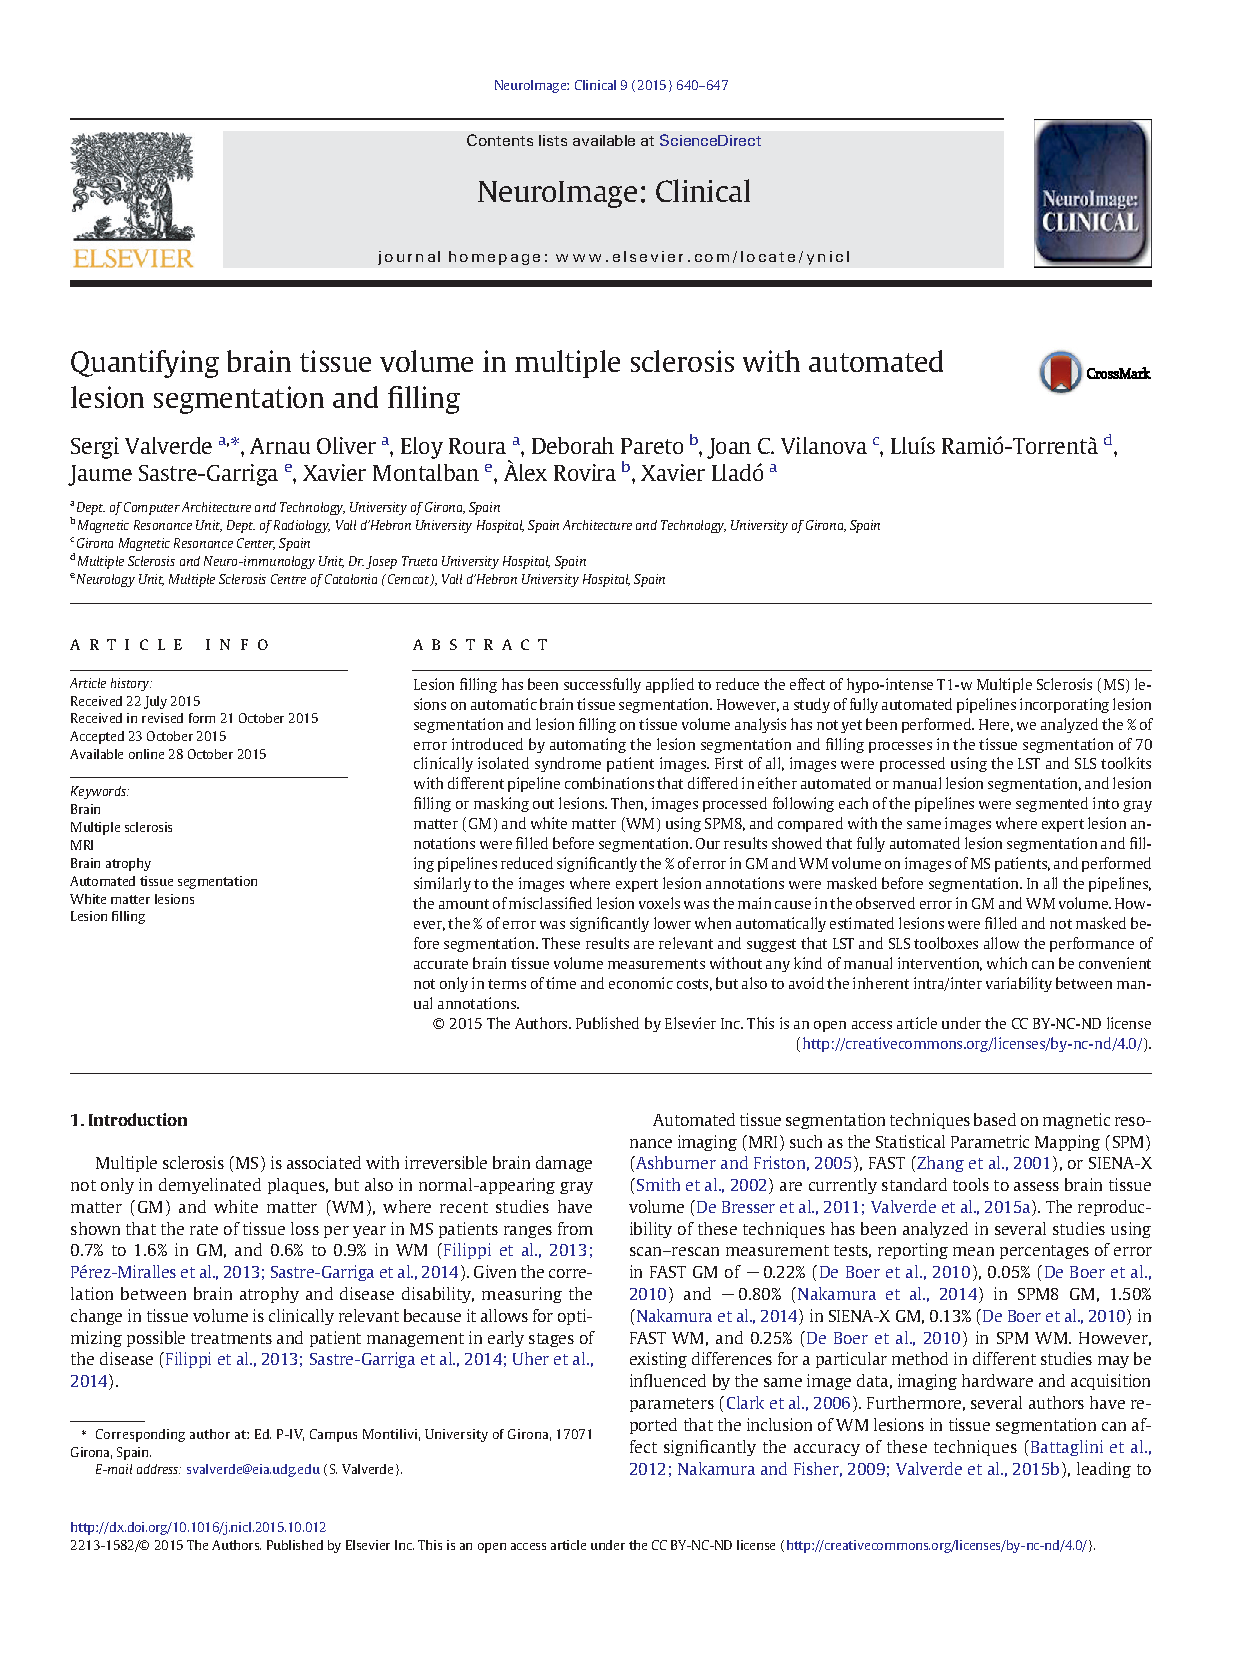
\includepdf[pages={-}]{./papers/nicl2015.pdf}


%%% Local Variables:
%%% mode: latex
%%% TeX-master: "../main"
%%% End:


